\section{Spectre}
Spectre vulnerability is entirely based on the exploitation of speculative execution.
When transient instructions are executed due to a wrong prediction, CPU is restored to its pre-prediction state, but many side effects remain unchanged, such as cache status, thus being one of the main side channels used for this attack, in particular the attacker might use Flush + Reload(x86 architecture supplies the clflush instruction for that purpose) or Evict+Time.
As we've seen different speculation techniques are used nowadays, increasing the attack surface.
This lead to the discovery of many variants, exploiting different techniques, using different side channels.
For this reason we won't go into too much depth for evry one of them, and will instead give a brief description of every variant.

\subsection{V1 - Conditional Branch Misprediction}
The first variant exploits conditional branch mispredictions, allowing the attacker to aribtrarily read from another context. As seen in the branch prediction section, when a conditional branch is encountered and a taken branch is predicted, the branch instructions are executed while checking for the condition.
Besides preparing the side channel the attacker must mistrain the branch predictor to make it execute transient instructions.
This can be achieved in different ways, like inserting a certain number of passed condition 
The attacker might use different conditions, with the most one being a bound check, and then accessing an array out of its bounds. When using this condition the attack is known as Bound Check Bypass.
The following is an example of this attack in C language:

\begin{Verbatim}[fontsize=\small]
if(x < array1_size)
	y = array2(array1[x] * 4096)
\end{Verbatim}

The ideal situation for the success of the exploit is such that array2 and array1\_size are uncached, even though in some scenarios the exploit works even if array1\_size is actually cached.
In this example the secret(array1[x]) is byte-sized, and array2 dimension is 1MB.
X is the offset from the starting address of array1 to the address we want to access.
The content of array2 in position array1[x] * 4096 (with 4096 being the size of a page) is cached.
To recover the secret value the attacker typically tries to access array2 in the 255 possible indexes and times every access.
Accessing the cached content will take way less clock cycles, and at that point the secret is easily recovered by dividing the array2 index by 4096.
The following is an example of this last described  method. We are assuming to run this instructions on a machine where the cache access time is at worst 50 cycles.

\begin{Verbatim}[fontsize=\small]
int max_cache_access_time= 50;
int secret;
for(int i=0; i<256; i++){
	current_clock= __builtin_ia32_rdtsc ();
	y = array2( i * 4096);
	spent_clocks=
	__builtin_ia32_rdtsc () - current_clock;
	if(spent_clocks<=max_cache_access_time){
		secret = i;
		break;
	}
}
\end{Verbatim}

\subsection{v2 - Branch Target Injection}
This variant exploits the Branch Target Predictor, in particular its ability to predict indirect branches.
The idea is mistraining the Branch Target Predictor in order to execute speculatively instrusction chosen by the attacker.
What the attacker does is finding functions contained in the libraries used by the victim program.
The concept is borrowed from Return Orienter Programming, a security exploit where arbitrary functions in a program are chained to together to execute what the attacker wants.
We will call this functions gadget just like in the just explained security threat.
To mistrain the Branch Target Predictor the attacker runs from its own context a program that reproduces the pattern of branches taken by the victim process before reaching the branch that must be mispredicted, thus exploiting the Branch Target Buffer.
How it must be mistrained varies among architectures, as the number of bit used per destination address changes.
After choosing the gadget, mistrainer we must branch to the same virtual address the predictor should mispredict to.
It doesn't matter what it's branching to, the goal is correctly mistraining the predictor.
This concept can be seen from Figure 7.

\begin{figure}[!h]
    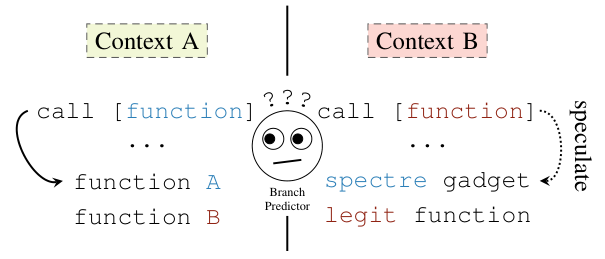
\includegraphics[scale=0.4]{img/sv2-mistraining.png}
    \caption{the attacker mistrains the predictor from his context(A), by jumping to a function that has the same virtual address as the gadget we want to be mispredicted in victim context(B)}
\end{figure}

We must also note that the mistrainer must run on the same core the victim program will run on, as prediction tables are not shared between different cores.
This is true for every type of predictor mistraining explained in this paper.
It has been proved that this attack allows to leak host memory from inside a guest Virtual Machine if the attacker has access to guest ring 0.

\subsubsection{Branch History Injection}
When Branch Target Injection first come out in 2018 Intel and ARM implemented respectively the eIBRS and CSV2 mitigations that prevent lower privilege programs from training the predictor into mispredicting branch target in higher privilege programs, by making the Branch History Buffer take into account the privilege the program is running in. 
We will better characterize these two mitigations later.
However at the beginning of 2022 researchers of the VUSec group have found another way to mistrain the Branch Target Predictor allowing cross-privilege mistraining, and called this technique Branch History Injection.
What they realized is that isolating Branch Target Buffer across different privileges is not enough, as the BTP relies on Branch History Buffer, that actually contains global entries.
From userland attackers can inject entries into the BHB and fill it with gadgets' address. When kernel-level progams are executed the predictor will base its prediction on the manually inserted entries, thut achieving cross-privilege mistraining.
Unlike BTI, AMD processors seem to be uneffected from this vulnerability, as only Intel and ARM CPUs are effected.

\subsection{SpectreRSB}
This variant of Spectre exploits the Return Stack Buffer, which job we have already explained in the Speculative Execution section.
The way this is exploitation is done is by polluting the RSB(i.e. manually injecting entries into it), in order to have the victim program execute gadgets the attacker has chosen.
Although not officialy adressed as an extension of Spectre v2, it uses an approach similar to the Branch HIstory Injection technique.

\subsection{v3 - Rogue Data Cache Load}
The third variant of Spectre is very rarely referred as Spectre v3, as it is more known as Meltdown. To deepen this topic, read Meltdown section.

\subsection{v4 - Speculative Store Bypass}
This last variant of Spectre, also known as SpectreSTL, exploits Speculative Store Buffer Bypass, allowing an attacker to read arbitrary priviliged data, or run older command speculatively than can lead to cache allocations, thus readable via common side-channel techniques.
